%!TEX root = ../thesis.tex



\chapter{Practical performences}
\label{chap:pracPerf}
\section{Setup}
\label{sec:Setup}
In the following chapter we will examine the practical relative performances of the three algorithms. We will do so in several ways. The first way is with the use of simulated data (recreated from \cite{Hastie2009}). We have ten features $X_1,\ldots,X_{10}$ which are drawn from a standard independent Gaussian. Their label is determined (deterministically) by the following rule: $$Y:=\begin{cases}
1 & \text{ if } \sum_{k=0}^{10} (X_k)^2 > \chi_{10}^2(0.5)\\
-1 & \text{otherwise}
\end{cases}$$ Where $\chi_{10}^2(0.5)=9.34$ is the median of a chi-squared random variable with ten degrees of freedom. This is to ensure that there roughly the same amount of labels in each category. 

\par The second way we will test the algorithms is the UCI ``a9a Adult dataset'' \footnote{https://www.csie.ntu.edu.tw/~cjlin/libsvmtools/datasets/binary.html}. Here the goal is to predict whether an individual will earn more than \$50,000 per year or not. The original data set has 14 features, among which six are continuous and eight are categorical. In this data set, continuous features are discretized into quantiles, and each quantile is represented by a binary feature. Furthermore a categorical feature with $m$ categories is converted to $m$ binary features. 

\par The final way we will attempt to compare the algorithms is to give them a fixed amount of CPU time and then compare the number of iterations they were able to do until the time elapsed and their accuracy at that point. Because of practical considerations we allow the algorithms to complete the current iteration when the time runs out, but since a single iteration doesn't take very long this should be of little concern.

\par In an attempt to keep the comparison as consistent as possible we will, in all settings, use 32,561 observations for training and 16,281 for testing. This is because these are the amount of observations in the a9a data set. This ratio of training to testing observations is not uncommon. Recall to avoid over fitting we cannot test the algorithm on the same dataset we use to train it, thus any observations which are used to test cannot be used to train, therefore this kind of ratio is desirable.

\newpage
\section{Datasets}
\subsection{\adaB}
\label{subsec:AdaPracPerf}
\begin{figure}[!ht]
  \centering
      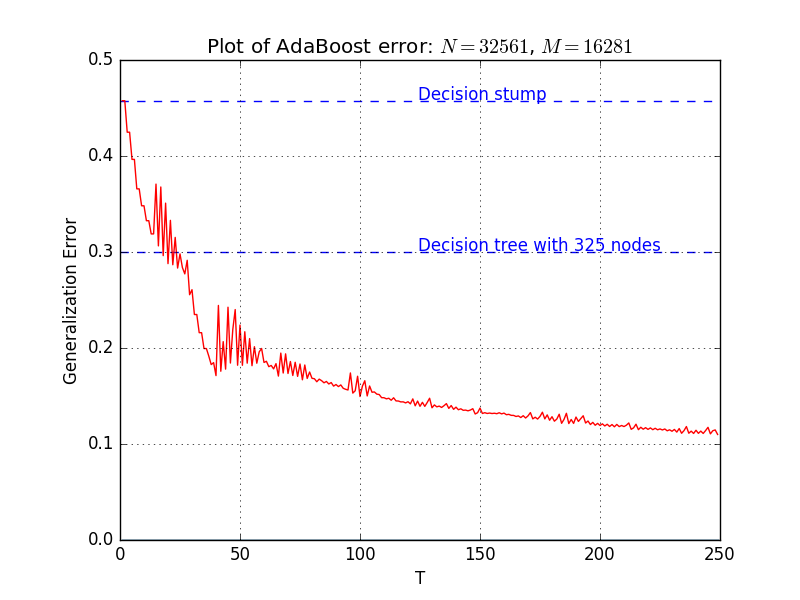
\includegraphics[width=\graphWidth]{generated/ADGD.png}
  \caption{Generalization error of AdaBoost as a function of the number of iterations over the simulated data set. The error rate of the decision stump and a decision tree with 321 nodes are shown for reference}
      \label{fig:adaBGD}
\end{figure}


\par Looking at figure \ref{fig:adaBGD} it is obvious that our algorithm works. The decision stump initially performs with an error rate of 47\% which is indeed only slightly better than random guessing. \adaB outperforms this and even a large tree with 321 nodes and an error rate of 30\% after just tens of iterations and reaches an error rate as low as 11\% after 250 iterations. 

\par Considering figure \ref{fig:adaBSVM} below the situation is a bit different for the a9a data. One sees that the algorithm still works but here we run into some limitations. As we can see the initial stump performs significantly better to start with, with an error rate of 23.6\%. After just 50 iterations we see diminishing returns set in quite drastically, seeing only a slight improvement from 15.7\% to 15.4\% over the course of 200 iterations. Of course this also happens with the simulated data but to a much lesser degree. This is probably due to the fact that the simulated data is much more homogeneous, where in fact all features are equally important, with the hard examples being those where all features are small but just meet the criteria. The observed data however most likely has a few features that improve the accuracy a lot (for example education), but beyond that the data doesn't show any important examples so the gains, after to low hanging fruit have been picked, are marginal. While this is still a good result it is useful to keep this phenomenon in mind while we examine the rest of the algorithms. This characteristic highlights a fundamental disadvantage of a weak learner, namely that depending on the data set there might simply not be a way to improve the accuracy beyond a certain point. 

\par A final observation on the reference trees should be useful here: while we did try to keep the size of the trees as consistent as possible, it is quite hard to enforce a specific size over different data sets, especially ones that differ as strongly as our two data sets. This is why the  trees have slightly different sizes across the different plots. We attempted to keep the sizes as similar as possible by enforcing a maximum depth of $\lfloor \log_2(500)\rfloor=8$, letting the algorithms fit the trees as best possible under this constraint. We have chosen this because this ensures an upper bound of 500 nodes, which we found to be a reasonable bound for the size and shapes of our considered data
\begin{figure}[!ht]
  \centering
      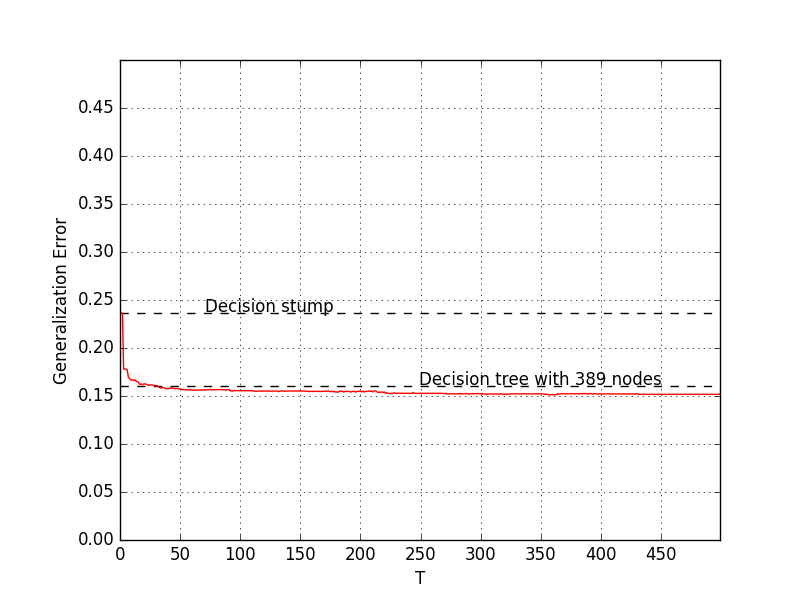
\includegraphics[width=\graphWidth]{generated/ADSVM.png}
  \caption{Generalization error of AdaBoost as a function of the number of iterations over the a9a data set. The error rate of the decision stump and a relatively large decision tree are again shown for reference}
      \label{fig:adaBSVM}
\end{figure}
\FloatBarrier

 \subsection{\NHB}
 \label{subsec:NHPracPerf}
Before we discuss the results of \NHB here we would like to highlight two important differences between \NHB and \adaB. The first is that to improve performance \NHB attempts to assign zero weight to unimportant examples. The percentage of examples which were assigned weight zero is shown in green in the plots below. The second important difference is that whereas \adaB decides the label based on a reference threshold, \NHB simply takes an unweighted majority vote. A consequence of this is that on the even iterations the final committee might be tied on a decision. In an attempt to reflect this in our comparison we count the inconclusive tests (shown in a percentage of the testing size in blue) and recorded these as ``half a mistake'' since the committee was neither right nor wrong. Of course this impacts the performance of the algorithm quite significantly as can be seen below.  One important remark is that the committees are never tied in the case of an odd size. For the sake of clarity the graphs of the inconclusive tests in the plots below only show the percentage on the even iterations, those on the odd iterations always being 0.


\begin{figure}[!ht]
  \centering
      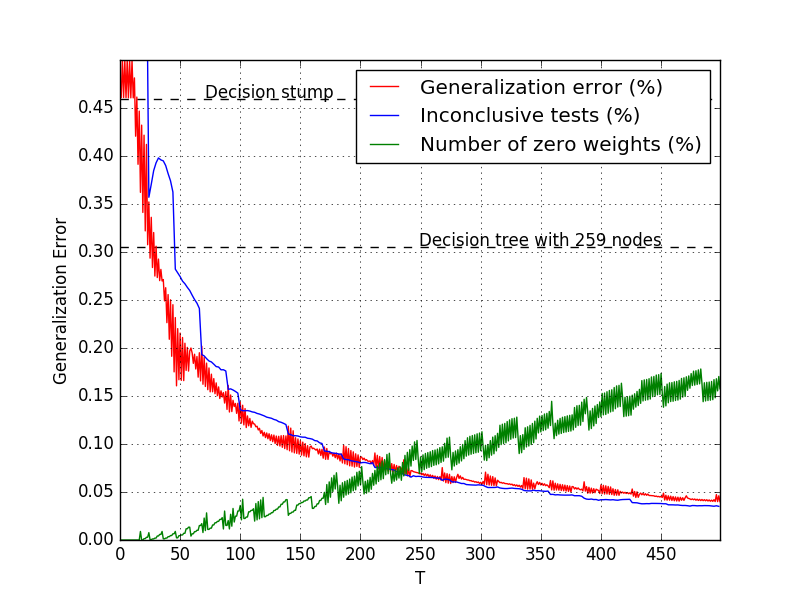
\includegraphics[width=\graphWidth]{generated/NHGD.png}
  \caption{Generalization error of \NHB as a function of the number of iterations on the simulated data. The error rates of trees with 3 and 259 nodes resp. are again shown for reference. It is important to remark that for clarities' sake we omitted the inconclusive data points of all odd iterations as they are always 0.}
      \label{fig:NHBGD}
\end{figure}
 \FloatBarrier
 \par The first thing one notices when looking at the above figure is that this mimics the behavior predicted by the theory, as well as the behavior of \adaB. The error rate as well as the percentage of inconclusive tests steadily decline while the percentage of zero weights steadily increase. In terms of actual percentages the algorithms perform quite similarly as was already studied in \cite{Luo2014}. Where \adaB achieved a error rate of 11.11\% after 250 iterations \NHB achieves 8.06\% which is slightly better. We will see however in section \ref{sec:timed} it is quite a bit faster. This is achieved by zero weight percentage of 8.47\% at the end. Since \NHB is the only algorithm that does this it isn't very useful for comparison's sake, but it is nice to see since it is quite a significant part which, again as we will see, improves performance quite a bit.  
\begin{figure}[!ht]
  \centering
      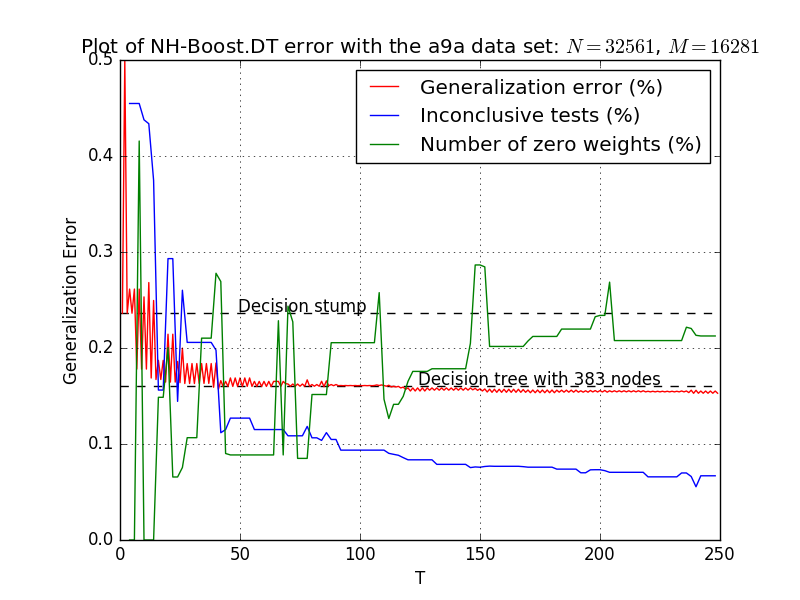
\includegraphics[width=\graphWidth]{generated/NHSVM.png}
  \caption{Generalization error of \NHB as a function of the number of iterations on the a9a data. The error rates of trees with 3 and 383 nodes resp. are again shown for reference. It is important to remark that for clarities' sake we omitted the inconclusive data points of all odd iterations as they are always 0.}
      \label{fig:NHBSVM}
\end{figure}

\par When looking at the observed data the story is again a bit different. The first obvious thing to note when looking at figure \ref{fig:NHBGD} is that the algorithm is (initially) quite confused about the amount of examples to assign a zero weight. One possible cause is that the weights of the previous round are determined by the performance of the previous iteration and that the algorithm gets slightly confused by the inconclusive tests. The peaks of zero weights are almost all around the 28\% whereas they last iteration has a zero weight percentage of 16.5\%. This compares quite favorably to the previous data set, which can be explained by our interpretation that after the low hanging fruit has been picked many examples become irrelevant and thus get assigned zero weight. One can, however, also wonder how reliable this interpretation is due to all the peaks and valleys. 
\par Here again we see the ``low hanging fruit'' characteristics we saw in the \adaB implementation. Here the final error rate bottoms out at 15.3\% compared to \adaB 15.4\% which is almost identical. One can wonder about the role the inconclusive tests play in this conclusion. This is however not of a big concern, since the accuracy on the odd iterations is also almost identical. Furthermore the inconclusive tests are an indication that the committee is not very certain on those predictions even if they aren't tied in the odd iterations. This tells us that these percentages are indeed very comparable.  
\FloatBarrier
\subsection{\squintB}
\label{subsec:sqPracPerf}
Finally we will consider \squintB. Looking at figure \ref{fig:SQGD} below we again see the predicted behavior. 
\begin{figure}[!ht]
  \centering
      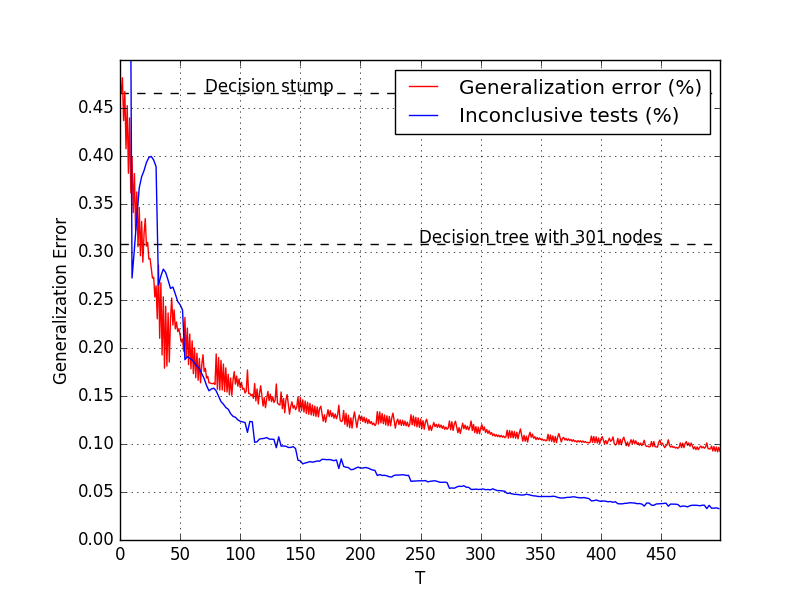
\includegraphics[width=\graphWidth]{generated/SQGD.png}
  \caption{Generalization error of \squintB as a function of the number of iterations on the simulated data. The error rates of trees with 3 and 301 nodes resp. are again shown for reference. It is important to remark that for clarities' sake we omitted the inconclusive data points of all odd iterations as they are always 0.}
      \label{fig:SQGD}
\end{figure}
\begin{figure}[!ht]
  \centering
      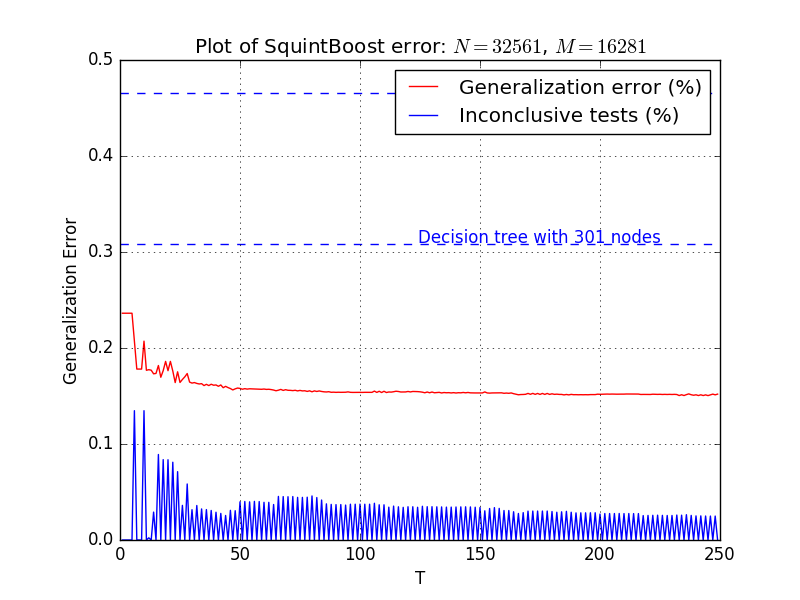
\includegraphics[width=\graphWidth]{generated/SQSVM.png}
  \caption{Generalization error of \squintB as a function of the number of iterations on the a9a data. The error rates of trees with 3 and 385 nodes resp. are again shown for reference. It is important to remark that for clarities' sake we omitted the inconclusive data points of all odd iterations as they are always 0.}
      \label{fig:SQSVM}
\end{figure}
\FloatBarrier

\newpage
\section{Computation}
\label{sec:timed}
\begin{table}[htbp]
\centering
\begin{tabular}{|c|c|c|c|c|}
\hline
Algorithm & Execution time (s) & Iterations & Error (\%) & Inconclusive tests (\%)  \\ \hhline{|=|=|=|=|=|}
\multirow{ 2}{*}{\adaB} & 1.194 & 5 & 39.64 & 0.00  \\\cline{2-5}
& 60.122 & 241 &  11.11 & 0.00  \\ \Xhline{1pt}
\multirow{ 2}{*}{\adaN} & 1.004 & 220 & 11.48  & 0.0 \\\cline{2-5}
& 60.000 & 15407 &  6.99 & 0.18  \\ \Xhline{1pt}
\multirow{ 2}{*}{\squintB} & 1.002 & 31 & 26.80  & 39.09\\\cline{2-5}
 & 60.022 & 1711 &  7.56  &  1.02\\ \hline
\end{tabular}
\caption{Timed tests of the algorithms on the simulated data}
\label{tbl:GDTime}
\end{table}

\begin{table}[htbp]
\centering
\begin{tabular}{|c|c|c|c|c|}
\hline
Algorithm & Execution time (s) & Iterations & Error (\%) & Inconclusive tests (\%)  \\ \hhline{|=|=|=|=|=|}
\multirow{ 2}{*}{\adaB} & 1.167 & 6 & 17.68 & 0.00  \\\cline{2-5}
& 60.192 & 297 &  15.25 & 0.00  \\ \Xhline{1pt}
\multirow{ 2}{*}{\NHB} & 1.085 & 12 & 17.80  & 0.0 \\\cline{2-5}
& 60.0120 & 578 &  15.14 & 0.0  \\ \Xhline{1pt}
\multirow{ 2}{*}{\squintB} & 1.024 & 15 & 17.93  & 9.23\\\cline{2-5}
 & 60.009 & 815 &  15.23  &  13.81\\ \hline
\end{tabular}
\caption{Timed tests of the algorithms on the a9a data}
\label{tbl:SVMTime}
\end{table}
{\huge\color{red}write about length of testing and diminishing returns in accuraccy with low hanging fruit}
\begin{table}[htbp]
\centering
\begin{tabular}{|c|c|c|}
\hline
Algorithm & Execution time (s) & Testing time (s)  \\ \hhline{|=|=|=|}
\multirow{ 2}{*}{\adaB} & 1.167 & 8.860 \\\cline{2-3}
& 60.192 & 414.593  \\ \Xhline{1pt}
\multirow{ 2}{*}{\NHB} & 1.085 & 92.030 \\\cline{2-3}
& 60.0120 & 6453.419  \\ \Xhline{1pt}
\multirow{ 2}{*}{\squintB} & 1.024 & 26.194\\\cline{2-3}
 & 60.009 & 1474.809\\ \hline
\end{tabular}
\caption{Testing time of the algorithms on the simulated data}
\label{tbl:GDTestingTime}
\end{table}

\begin{table}[htbp]
\centering
\begin{tabular}{|c|c|c|}
\hline
Algorithm & Execution time (s) & Testing time (s)  \\ \hhline{|=|=|=|}
\multirow{ 2}{*}{\adaB} & 1.167 & 24.160 \\\cline{2-3}
& 60.192 & 1038.695  \\ \Xhline{1pt}
\multirow{ 2}{*}{\NHB} & 1.085 & 38.211 \\\cline{2-3}
& 60.0120 & 1829.719  \\ \Xhline{1pt}
\multirow{ 2}{*}{\squintB} & 1.024 & 1.024\\\cline{2-3}
 & 60.009 & 1870.409\\ \hline
\end{tabular}
\caption{Testing time of the algorithms on the simulated data}
\label{tbl:SVMTestingTime}
\end{table}
\FloatBarrier
 \section{Conclusion and Future Work}
 \label{sec:Concl}